\chapter{Experiments}
In the previous chapter we have outlined all the important steps in the process of constructing Vector 
Space Models, and listed all major approaches that we thought to be important for the task of Word 
Sense Disambiguation. There are certainly many other approaches that are employing VSM in some CL 
or NLP task, but because their domain of application is not relevant for the task of interest they where not 
mentioned here. This chapter is devoted to describing the full methodology behind the experiments 
performed in this thesis as well as how this methodology stems from previous approaches in VSM, 
in all the relevant phases of the process. First we will describe the resource that WSD was performed on, 
Prague Dependency Treebank, which will be followed with data preprocessing section. In the section 
after we will describe all the models implemented for the WSD task. After that the evaluation rationale 
will be presented. All experiments were performed on the principle: one model-- one experiment. In the 
final sections of this chapter results of experiments with the baseline random guessing scores will be 
 presented.


\section{The resource}
Prague Dependency Treebank (PDT) is  project that stemmed from work of a group of Czech linguists 
(Institute of Formal and Applied Linguistics\footnote{http://ufal.ms.mff.cuni.cz/}, Institute of Theoretical 
and Computational  Linguistics\footnote{http://utkl.ff.cuni.cz/}) from Charles 
University\footnote{http://www.cuni.cz/} in Prague and Masaryk 
University\footnote{http://www.muni.cz/}  in Brno. PDT was  inspired by the research resulting from the 
Penn Treebank\footnote{http://www.cis.upenn.edu/~treebank/} project. 

PDT was generated in two major phases. In the first phase (1996--2000), the morphological and syntactic analytic  layers of annotation have been completed along with the preview of tectogrammatical layer annotation available as  PDT 1.0. During the second phase (2000--2004), the tectogrammatical layer of annotation was completed and PDT 2.0 was done.
\\The structure of Prague Dependency Treebank (PDT) consists of three layers:
\begin{itemize}
\item morphological layer (lowest)-- full morphological annotation
\item analytic  layer (middle) -- superficial (surface) syntactic annotation using dependency treebank; level conceptually close to the syntactic annotation used in the Penn Treebank 
\item tectogrammatical layer (highest) -- level of linguistic meaning
\end{itemize}
In our experiments we were using as a resource PDT 1.0 version, instead of PDT 2.0. Frequencies for each layer in PDT 1.0. are given in the table below:
\begin{table}[h!]
\begin{center}
	\begin{tabular}{ l  c  | c c }
   	&    & \# of tokens & \# of sentences \\
	\hline                       
	& morphological (total) & 1,725,242 & 111,175\\
	& syntactic--analytic (total) & 1,507,333 & 98,263 \\
  	& tectogrammatical (portion) & 3,490 &  203 \\
	& morphological and syntactic--analytic & 1,255,590 & 81,614 \\
	\end{tabular}
\end{center}
\caption{Frequencies of tags for every layer in PDT 1.0.}
\end{table}
\\\\\\\\
\textbf{Text Sources}
\\\\The text material that was annotated in PDT contains samples from the following sources:
\begin{itemize}
\item Lidov\'e noviny\footnote{http://www.lidovenoviny.cz/} (daily newspapers), 1991, 1994, 1995
\item Mlad\'a fronta Dnes\footnote{http://www.idnes.cz/} (daily newspapers), 1992
\item Ceskomoravsk\'y Profit (business weekly), 1994
\item Vesm\'ir (scientific magazine), Academia Publishers, 1992, 1993
\end{itemize}

\subsection{Polysemous words}\label{pdt}
Czech language is the typical representative of inflectionally rich free--word--order language\footnote{http://www.czech--
language.cz/index.php}, which surely doesn't have a favorable influence on the number of polysemous words in Czech 
language. From the training set that represents approximately 9/10 of the whole PDT 1.0 we present in the table below the 
number of words that have more than one meaning. In the left column is given the number of meanings, and in the right column 
the number of words that take that number of meanings. For instance, the eight row informs us that there are two words that 
take 8 different meanings in the training set. It has to mentioned that these numbers could be different in another instance of 
training, being that the training set is assembled pseudo--randomly before the training phase. However, for the PDT training set they would not be drastically different because training is performed on the 90\% of the entire set. 
\begin{table}[h!]
\begin{center}
	\begin{tabular}{ c  c |  c }
   	&   \# of meanings & \# of types \\
\hline  
 & 2 & 319  \\
 & 3 & 49  \\
 & 4 & 19  \\
 & 5 & 9  \\
 & 6 & 5  \\
 & 7 & 1  \\
 & 8 & 2  \\
\hline  
& &Total =404\\  
 	\end{tabular}
\end{center}
\caption{Number of types with multiple meanings in the training set}
\end{table}



\subsection{Why PDT 1.0 instead of PDT 2.0?}
The question from the title of the section is indeed a perfectly valid and reasonable question indeed, for 
any type of research-- why use an older version of a resource, when there is a newer, more complete 
version of the same resource?  

To answer this question we must go back to the task that is in focus of this research. For the WSD task the 
important feature of the text on which the system is trained and tested on is that every different meaning of a 
word is marked orthographically different. This information that could be extracted both from PDT 1.0 and 
PDT 2.0, therefore for the WSD task one resource is as much sufficiant as the other one. The only 
difference between the two treebanks is that PDT 2.0 contains additionally the tectogramaticall layer, that 
was not used in this research.  

When building(training) Vector Space Models, a researcher might want to include POS information with 
every tag. This was not done in our experiments but it was always an option supported by the resource, 
because like previously mentioned, PDT 1.0 is fully annotated on the syntactic level. 
%\\On top of these reasons, another incentive that made us decide for PDT1.0 is that it essentially represents a light--wight version of PDT2.0, encoded in Standard Generalized Markup Language (SGML\footnote{http://www.w3.org/MarkUp/SGML/}), which made it easier to handle during the preprocessing stage.

\section{Preprocessing}
The preprocessing phase involves several several sub--stages. As we have described theoretical approaches to these steps in length in previous chapters, we have decided to explain all the preprocessing steps performed in experiments in this chapter. Preprocessing involves following sequential steps: text extraction from PDT files along with relevant tags, text normalization, stemming and filtering. 
\\\\  \textbf{Text extraction}

Text used during training and testing phase of VSM was extracted from PDT files and put into a single file. 
In order to make the implementation applicable for other resources other than PDT we have made a 
design decision that the implementation uses this single file as its input. Apart from the single--meaning 
words, the system extracts multiple meaning words, and represents differently each separate meaning. In 
PDT1.0 if a word has multiple meanings, meaning of that word is given in a separate tag, in the following format: 
\textit{word--index\_number\_of\_meaning}. Index number increments as the word has more meanings.

Therefore, the tagging step in this case was simplified: \textit{every multiple--meaning word was 
represented with its orthographic representation meaning in context}, which was simply extracted from 
the Treebank. An example of a sentence extracted from PDT is given below:
\begin{examples}
\item Krumbachov\'a pr\'aci p\v{r}ijmout--2 podle--2 vlastn\'i--1 slov " v--1 hodin\^e dvan\'act\'e ".
\glt \textit{ Krumbach has accepted the work " in the last minute" .} 
\end{examples}
Word's meaning in context was given as it was represented in PDT.
\\\\  \textbf{Text normalization}

Czech language has spelling variants-- words that are orthographically slightly different but are actually 
identical on every other level of analysis, for example words like \textit{abch\'azsk\'a}  and 
\textit{abchazsk\'a}. Many foreign names have variant spellings, especially in marking the vowel length. 
Spelling variants should not be counted as different types so it was therefore decided to normalize all 
characters with diacritics marking the vowel length into characters without them. 
\\As a measure of normalization that would reduce distributional sparsity of words all words were 
lowercased. Punctuation marks were also filtered from the entire corpus, so that the models could be 
trained on terms only. 
\\\\  \textbf{Stemming}

Stemming process was detailed in the Chapter \ref{linguisticPreprocessing}, as well as how it is different 
from lemmatization. To re--iterate: lemmatization is more precise than stemming because it picks up 
lexical variants that are not orthographically similar to the stem. At the same time it is much harder to 
implement than a stemmer, because it requires utilization of a lexicon. 

Although a good lemmatizer was built at 
UFAL\footnote{http://ufal.mff.cuni.cz/pdt/Morphology\_and\_Tagging/Morphology/index.html}, it was not 
used 
in this system. During preliminar experiments with cosine-weighted co-occurrence matrix it was observed 
that the improvement in precision when applying lemmatizer over stemmer is not significant. It was 
therefore
assumed that precision would not be improved in other models experimented with as well. 
A stemmer built for the Czech language made at University of 
Neuchatel\footnote{http://members.unine.ch/jacques.savoy/clef/CzechStemmerLight.txt} was used in 
preprocessing 
phase.  An example of text that 
was extracted, normalized and stemmed is given below:
\begin{examples}
\item krumbach prak p\v{r}ijmout--2 podle--2 vlastni--1 slov " v--1 hodin dvanact ". 
\glt \textit{  Krumbach has accepted the work " in the last minute"  .} 
\end{examples}
In example above we can see how a brute force of stemming can sometimes fail because it does not employ linguistic analysis. Czech noun  \textit{pr\'ace}, here in its inflected form \textit{pr\'aci} has fallen under a stemmer's rule for palatalisation which converts endings like \textit{--ci, --ce, --\v{c}i, --\v{c}} into \textit{--k}, which is wrong. However, as later experiments will prove, this does not affect the algorithm's precision in a bad way.  
\\\\  \textbf{Word Filtering}
\\Two effective filtering criteria were applied (optionally) in our experiments for the purpose of reducing the sparsity of vectors and improving overall precision: POS and low frequency counts. A list of Czech stop words was compiled(Apendix A) in order to filter out words that belong to closed grammatical classes. Both types of filtering were experimented with, in order to observe how their tunning influences the overall precision of system.

\section{Train and test sets}\label{trainTestSet}

After extracting the text from PDT and optional preprocessing normalization performed on text, text's 
sentences are randomized and split into 3 separate files: $train, testDev, testFinal$. Training set holds 
90\% of the number of sentences in the whole set, while $testDev$ holds about 5\% and $testFinal$ 
about 5\%. First test file 
($testDev$) is used to evaluate during training phase, while the second ($ testFinal$) is used for 
evaluation in the testing phase. 

Below is given an overview of the number of types and tokens for each of these files, before and after 
preprocessing applied to them:

\begin{table}[h!]
\begin{tabular}{ l | c c | c c | c c|}
& \multicolumn{2}{|c}{train set} & \multicolumn{2}{|c}{test devel set} & \multicolumn{2}{|c|}{final test set} \\
   &  \#types & \#tokens  &  \#types & \#tokens  &  \#types & \#tokens \\
  \hline                       
no preprocessing &138098 & 1521180 & 6447 & 20536 & 19858 & 80514 \\ 
 merge variants &137448 & 1521180 & 6444 & 20536 & 19824 & 80514 \\ 
stemming &71311 & 1521180 & 4965 & 19054 & 20536 & 80514 \\ 
\end{tabular}
\caption{Influence of the preprocessing method on the size of training and test token count}
\end{table}
We can observe that stemming reduces the vocabulary size much more than merging 
lexical variants. This fact will reflect on the precision in the evaluation phase. The number of types decreases with the application of an individual normalizer, while the number of tokens stays the same in all sets. 

\section{Document size}
After preprocessing phase, the next step is to build the term--document matrix. This step is generalized for all the models we will be training. This is because the term--document matrix is a simple frequency matrix, and (optional) normalization of frequency counts or dimensionality reduction takes place in the next phase. Crucial property of this phase is the size of the document in the term--document. Previous approaches were described on the use of context, ranging from word--level to paragraph--level. Document size used in the following experiments will be: 
\begin{itemize}
\item five sentence paragraph
\item three sentence paragraph
\item one sentence paragraph
\item three neighboring words of preceding and succeeding context
\item two neighboring words of preceding and succeeding context
\item one neighboring word of preceding and succeeding context
\end{itemize}
To further clarify what exactly do last three items in the list mean, we will point out that the since the task
at hand is disambiguation of polysemous words. Therefore, polysemous meanings should be in focus of
every document. We have decided to conduct experiments by partioning sentences into fragments where 
in the center of every such fragment is a polysemous meaning, surrounded by symmetrical window 
length of varying size. An example is given for a one neighboring word of preceding and succeeding context. For a sentence:
\begin{examples}
\item Krumbachov\'a pr\'aci p\v{r}ijmout--2 podle--2 vlastn\'i--1 slov " v--1 hodin\^e dvan\'act\'e ".
\glt \textit{  Krumbach has accepted the work " in the last minute" .}
\end{examples}
the corresponding fragments extracted from it are:
\begin{examples}
\item pr\'aci p\v{r}ijmout--2 podle--2
\item p\v{r}ijmout--2 podle--2 vlastn\'i--1
\item podle--2 vlastn\'i--1 slov
\item slov v--1 hodin\^e
\end{examples}
This kind of fragmentation increases the number of documents in the co-ocurrence matrix. The rationale behind this was that centering documents around polysemous encounters will help in training the model to be better. The idea was that in this way the model will become ''more sensitive" for contexts in which the ambiguous words appear, and will assign correct meanings to their rightful contexts better. 

Choice of document size during model training is one of the crucial features of VSM, and can very much 
influence the results of the model's performance, through the size of vocabulary. Size of vocabulary is 
influenced by 
preprocessing method applied as well the size of the document. Below is given a table that shows how 
the choice of document size influences the size of vocabulary, for the corpus that was not preprocessed. 

\begin{table}[h!]
\begin{tabular}{ l | c | c c |c c}\label{docSize}
			& \#index  &  ambiguous  words && other words \\
 document size & documents & \#types & \#tokens & \#types & \#tokens \\
\hline
5 sentences & 15732 & 3513 & 4721 & 128676 & 1155781\\
3 sentences & 26220 & 3334 & 4417 & 129618 & 1166559\\
1 sentence & 78660 & 2116 & 2660 & 130620 & 1216412\\
3+3 & 231673 & 2116 & 2660 & 105225 & 1433731\\
2+2 & 231673 & 2116 & 2660 & 94018 & 1088417\\
1+1 & 231673 & 2116 & 2660 & 70772 & 700799\\
\end{tabular}
\caption{Influence of document size on the volume of vocabulary}
\end{table}

With the word--level document size we can observe that number of types is smaller than in sentence
--level documents. This is due to existing gaps between documents in matrix with word--type document.
Number of tokens  can be bigger which we see in the case of 3+3 document size, because in some 
places, where two occurrences of ambiguous words stand next to each other, there will be an overlap
which will be counted. 

\section{Normalization of the frequency counts and dimensionality reduction}
Normalizing the frequency counts was done in two ways in experiments: the traditional TF--IDF weighting, and the enthropy--based weighting as prescribed in LSA. To re--iterate the formulas again:
 \begin{center}
\begin{equation}\large{f_{ij} = TF_{ij} \cdot DF_{i} \cdot S_{j}}
\end{equation}
\end{center}
,where $TF_{ij}$  is the frequency of term \textit{i} in document \textit{j}, $DF_{i}$ is some function of the number of documents term i occurs in (DF for \textit{document frequency}), and $S_{j}$ is a normalizing factor, usually dependent on the length of document(s for scaling).
DF is usually computed as:
\begin{center}\large{
\begin{equation}IDF = log \frac{D}{DF_{i}}
\end{equation}
}
\end{center}
, where D is the total number of documents in the whole corpus. 
%\todo{
%++Keyword Density Values
%\begin{large}
%$ KD_{i} = \frac{tf_{i}}{L_{i}}  $
%\end{large}
%}
\\\\  
Another frequency weighting performed was the entropy--based weighting as given in the formula below:
\begin{center}\large
\begin{equation}E_{ij}=1+  \frac{\sum_{j}{P_{ij}log P_{ij}}}{logD}
\end{equation}
\end{center}
where \textit{D} is the total number of documents in the collection. $P_{ij}$ is given with a formula
\begin{equation}\large{P_{ij} = \frac{TF_{ij}}{f_{i}}} \end{equation}
where $TF_{ij}$ is the frequency of term $i$ in document $j$ and $f_{i}$ is the frequency of term \textit{i} in the whole document collection.

The last model that was experimented with is created through the use of dimensionality reduction 
technique-- Random Indexing. Frequencies counts of its term--document matrix were not normalized, 
due to the nature of its generation. Detail description of RI is given in chapter\ref{RI}. What should be 
restated is that:
\begin{itemize}
\item It builds term vectors by adding pseudo--random vectors assigned to documents in the corpus.
\item It uses fixed dimensionality for both term and document vectors, which means that new data do not 
increase the dimensionality of the vectors.
\item It uses implicit dimensionality reduction, since the fixed dimensionality is
much lower than the number of contexts in the data. Producing
context vectors with RI is only $O(wr)$, since the method is not reliant on the
initial construction of the co-occurrence matrix.
\item It is incremental, which means that the context vectors can be used for similarity
computations even after just a few examples have been encountered.
\end{itemize}
More details on RI can be found in Chapter\ref{RI}. 

The two approaches to weighting the co--occurrence matrix(TF--IDF and PMI) and one approach to 
dimensionality reduction (RI) are considered as fundamentally different. That is why the experiments are organized around these models, with other 
parameters like preprocessing, document size, and evaluation context size and number of word 
meanings threshold used in the evaluation(both explained in following sections) are changed to investigate how they influence the overall performance. 

\section{Evaluation context size} 
After the co-occurrence matrix is built and frequencies of its elements are normalized with some 
value (TF--IDF or PMI), or the matrix's dimensionality is reduced (RI) our model is ready to be tested out.
This means that now for every word in the dictionary we have a vector that is in a way its representation.
A unique methodology is then applied for each model in order to calculate the measure of appropriateness for a current word meaning against the context it is found in. Size of the context around the current meaning in question is experimented with and in our experiments takes values from 1 to 7, to determine the influence of symmetric context size on the overall accuracy. 
Evaluation context size is the number of words taken from preceding and succeeding context of the 
occurrence of ambiguous word. For instance, for the sentence:
\begin{examples}
\item Krumbachov\'a pr\'aci p\v{r}ijmout--2 podle--2 vlastn\'i--1 slov " v--1 hodin\^e dvan\'act\'e ".
\glt \textit{ Krumbach has accepted the work " in the last minute"  .}
\end{examples}
, corresponding contexts for the evaluation context size set to 1 extracted from it are:
\begin{examples}
\item p\v{r}ijmout--2 : pr\'aci  podle--2
\item  podle--2: p\v{r}ijmout--2 vlastn\'i--1
\item podle--2 slov
\item slov  hodin\^e
\end{examples}


In the implementation level, the way the most appropriate meaning for the context is calculated in two passes:
\begin{itemize}
\item The test set is traversed, in order to extract all the contexts for all the polysemous words 
encountered  in testing.
\item Extracted contexts are traversed, and for every different meaning the appropriateness for that 
word meaning in context is calculated. The meaning that has the highest score is selected as the 
true meaning by the system.
\end{itemize}  
Two things here are of importance: the way context vectors is built, and the way distance between context vector and meaning vector is calculated. Context vector in all cases (TF--IDF, PMI and RI) is 
built by superposition of all the term vectors constituting that context. If the term was not encountered 
during training it is skipped. If context vector does not have any terms inside it then that context is skipped during evaluation. This means a difference in size of vocabulary made in training can influence the number
of contexts being evaluated, and therefore the test set size. 

Distance between context and 
meaning vector is calculated as a cosine distance in all cases.

To repeat, cosine distance is  the angle between two vectors $\vec x$ and $\vec y$, defined as:
\begin{center}
\large{
\begin{equation}sim_{COS}(\vec x ,\vec y) =  \frac{\sum_{k=1}^n x_{i}y_{i} }{\sqrt []{\sum_{k=1}^n x_{i}^{2}} \sqrt []{\sum_{k=1}^n y_{i}^{2}}} 
\end{equation} 
}
\end{center}

\section{Evaluation metrics and baselines}
In this section evaluation metrics and baselines used in this research will be presented, employed for 
\textit{in vitro} evaluation of WSD systems (Navigli 2009). The evaluation the WSD system as a module 
embedded in applications (called \textit{in vivo} or \textit{end-to-end} evaluation) was not conducted 
in this research.  
\\\\
All sentences extracted from the PDT and annotated to distinguish different meanings of polysemous
words are divided into three sets (files): training, test development, and test final. Training takes about
9/10 of the entire set, while the rest is distributed evenly between two test sets. During the training 
phase the model is trained on the training set, and evaluated on the test development set. In the evaluation
phase training and test development sets are merged, the model is trained on them, and evaluated on the
final test set, which represents the unseen portion of data. This ensures an unbiased evaluation of every
model.
\\\\
Given the individual training and test sets \textit{coverage C} is defined as the percentage
of items in the test set for which the system provided a sense assignment:
\begin{equation}
\large{C=\frac{\#answers\_provided}{\#total\_answers\_to\_provide}=\frac{TP+FP}{TP+FP+FN}
}
\end{equation}
\\\\
If the systems provides an answer for every test instance then $C=1$.
The \textit{precision P} of a system is computed as the percentage of correct answers given by the 
system. If the model ''calculates the correct meaning" properly, 
\\$\#correct\_answers\_provided$ is 
incremented. The total number of answers given by the system is counted as well, and then precision 
is calculated as: 
\begin{equation}
\large{P=\frac{\#correct\_answers\_provided}{\#answers\_provided}=\frac{TP}{TP+FP}
}
\end{equation}
%TODO REMOVE TP, FP, FN BECAUSE THE DEFINITIONS ARE NOT THE SAME IN WSD
\\\\
Precision determines how good are the answers given by the system.
\textit{Recall R} is defined as the number of correct answers given by the automatic system
over the total number of answers to be given:
\begin{equation}
\large{
R=\frac{\#correct\_answers\_provided}{\#total\_answers\_to\_provide}=\frac{TP}{TP+FP+FN}
}
\end{equation}
\\\\
If the coverage of the system is absolute ($C=1$) then recall and precision will be equal. 
From these two values (precision and recall) an F--measure is calculated according to formula:
\begin{equation}
\large{
F-measure=\large{\frac{1}{\frac{\alpha}{P}+\frac{1-\alpha}{R}}}
}
\end{equation}
where $\alpha$ is the weight factor which in experiments performed here takes the value of 0.5, in order to give equal weights 
to both precision and recall. As it is customary for WSD experiments (Navigli 2009), all results in the experiments are presented in 
as Precision/Recall pairs, though an alternate output in the form of F--measure/Coverage could be enabled as well by the 
system.   
\\\\
\textbf{Baseline.}

As a baseline result, random guessing is calculated for every test set used in evaluation. Random baseline is the probability of a 
random choice of a sense from those available for each polysemous word $w_i$ . Overall random 
precision is then calculated as:
\begin{equation}
\large{
RandomP=\frac{1}{n} \sum_{i=1}^{n}\frac{1}{Senses(w_i)}
}
\end{equation}
where $Senses(w_i)$ is the number of senses that a $w_i$ can have. 

\section{Tuning}
Number of meanings that polysemous words encountered in the corpus can vary from 1 to 8 meanings. The actual number of meanings follows Zipf's distribution, where ranks are the number of meanings word 
can take (1 to 8) and numbers are the number of polysemous words that take that number of meanings. 
To illustrate this with a simple example: number of words that take 2 meanings in PDT 1.0 is 329. 
Full table is given in chapter \ref{pdt}.In the figure 6.1 is given a plot to illustrate how meaning's counts and word 
types conform to the Zipfian distribution.

\begin{figure}[h!]
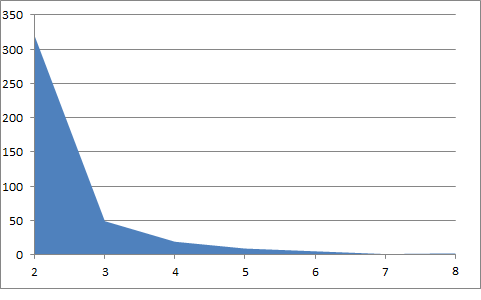
\includegraphics{img/meaningTypePlot2.png}
\caption{Distrubution of number of polysemous types per number of meanings}
\end{figure}


Three types of experiments for each model were performed, in order to tune each model to achieve its 
best performance.
\subsection{Tuning preprocessing parameters}
Each of the preprocessing measures mentioned before 
(lowercasing, filtering words that belong to the closed class group, stemming and merging of lexical
variants in Czech language) was experimented against the different document size (5,3,1 sentence 
document and 3+3, 2+2, 1+1 words surrounding polysemous word) to determine for which parameters the model achieves the highest accuracy. These models were evaluated only for highly polysemous
words, at the fixed size of the evaluation context size. In  order to able to test how models really perform 
we train models only on highly polysemous words, the ones that have 5 or more meanings.  For instance, there are 19 
polysemous words in the test development set that can take 5 to 8 meanings.

\subsection{Tuning evaluation context size} 
When the best parameters for preprocessing and document size (in the term--document matrix) are 
discovered, the next tuning phase experiments with different sizes of Evaluation Context against these best 
paremeters. There are two motivations for this sequence of tuning experiments: first, the preprocessing
 and building the matrix come before matrix frequency normalization and evaluation. Second, after
the best parameters in the preprocessing stage are found, we can observe how this (best) model behaves 
with different sizes of context (from which the evaluation context vector is constructed). 

\subsection{Evaluation on polysemous words of different level } 
Words whose orthographic representation can take on a large number of meanings can be considered
as ''highly polysemous", while words that can take on a small number of meanings(like two or three) can 
be regarded as ''not highly polysemous". As explained, numbers of occurrences of polysemous words 
conform to the Zipfian distribution, which means that there is only a small number of highly polysemous
words. Therefore, when experimenting with such words test set is not overly large, but if other, less
polysemous words are included, the number of test set instances rise. The purpose of this experiment
is to investigate how do models handle more and less polysemous words. Ranges from 2 to 8 meanings per word
are taken into consideration.

\newpage
\section{TF--IDF experiments}
As previously mentioned experiments are organized around 3 different different Vector Space Models, 
based on the weighting of the matrix elements or dimensionality reduction technique. Matrix reduction technique used for this model was TF--IDF (described in Chapter 6.5). For all the models experiments were performed on every parameter for a range of meaningful values. Parameters are grouped according to the phase in which they were used in:
\begin{itemize}
\item Tuning preprocessing parameters (preprocessing method and document size in co-occurrence matrix)
\item Tuning evaluation context size 
\item Evaluation on polysemous words of different level
\end{itemize}
These rounds are ordered sequentially in order to ensure best possible tuning for the model. Final step
represents an evaluation on words with different degree of ambiguity attached to them.

\subsection{Tuning preprocessing parameters}
First, no preprocessing method was applied on the train and test set. The size of the document in the term--document co-
occurrence matrix was changed in order to observe the influence on the precision. A threshold number of meanings to be evaluated on was set to 5, which means that other polysemous words that had less than 5 meanings encountered in training were discarded for this test. There was 177 polysemous words that appeared in 1861 occurrences, and for this test set a number of test instances was discarded for having a 
low number of meanings. The reason for discarding is that this round of tests is aimed at finding the best preprocessing method, so therefore a full number of test instances was not necessary.  
 An evaluation context size was fixed to 3, which means that a symmetric window 3 preceding and 3 succeeding words were used to build a vector which was used for classification. First column in the table displays the preprocessing method used on the entire corpus (except on the test instances) used in the phase of constructing co--occurrence matrix. To ensure that the best preprocessing method is chosen, regardless of the 
document size used in co--occurrence matrix, different size of documents were observed. Document sizes that were
experimented with are: 5 sentence document, 3 sentence document, 1 sentence document, and 3+3, 2+2, 1+1 symmetric word windows around polysemous word.  
For baseline random precision was calculated for every individual test. Random precision represents the precision of the system when it is picking a random meaning for a polysemous word that is tested. 
Precision and recall (in \%) for every document size is presented in the tables below. First a sentence--level 
document size was experimented with. This means that for the units from which the frequencies were calculated from (for the co-occurrence matrix) the paragraphs of size 1, 3 and 5 sentences. 
Best results in all the tables are bolded. 

\begin{table}[h!]
\begin{tabular}{ l | c c | c c | c c | c}
   preprocessing &  1 sentence && 3 sentences && 5 sentences  && random\\
\hline
	& P  &  R & P  &  R & P  &  R & precision\\
\hline\hline
 NO  & 92.31 & 100 & 94.57 & 100 & 95.67 & 100  &11.36 \\
LOWCASE  & 90.6 & 100 & 91.45 & 100 & 92.31 & 100 & 11.36 \\
STOP  & 89.74 & 100 & 93.16 & 100 & 94.87 & 100 & 11.36 \\
 STEM  & 90.6 & 100 & \textbf{96.58} & 100 & 95.73 & 100 & 11.36 \\
 MERGE  & 90.6 & 100 & 94.87 & 100 & 95.72 & 100 & 11.36 \\
\end{tabular}
\caption{Precision and Recall using various individual preprocessing techniques, sentence level document size}
\end{table}

Random precision is the same regardless of the preprocessing technique applied due to the fact that 
they were applied to all tokens except the polysemous words. This had helped preserve the size of the 
test set, which reflected on the consistent number of random precision in tests. Recall is 100 because all test instances were encountered in training and the system was able to
provide an answer. This is not necessarily always the case, it depends on the pseudo--random split on 
training and testing sets  whether an instance will be encountered during training. 
\\\\
It seems that individual 
 preprocessing technique that yields best results is stemming, though lowercasing and merging of Czech variants give the most consistent results. To ensure the validity of these findings, same test was repeated for the word--level document size. Results are given in the table below.  
\begin{table}[h!]
\begin{tabular}{ l | c c | c c | c c | c}
   preprocessing & 1+1 word && 2+2 words && 3+3 words  && random\\
\hline\hline
	& P  &  R & P  &  R & P  &  R &\\
\hline
NO  & 90.6 & 100 & 94.87 & 100 & 95.73 & 100 & 13.96 \\
LOWCASE  & 91.45 & 100 & 95.73 & 100 & 95.73 & 100 & 13.96 \\
 STOP  & 89.74 & 100 & 93.16 & 100 & 94.87 & 100 & 13.96  \\
 STEM  & 90.6 & 100 & 96.58 & 100 & 95.73 & 100 & 13.96 \\
MERGE  & 93.58 & 100 & 98.17 & 100 & \textbf{98.17} & 100 & 13.76  \\
\end{tabular}
\caption{Precision and Recall of TF--IDF model, no preprocessing, word level document size}
\end{table}

Evaluation of preprocessing technique on the word level document size gives approximatively similar results, though it can be observed that merging of Czech variants gives slightly better results in this case. Lowercasing filtering of Czech stop words is not that far behind. In the next round of experiments, combinations of best individual techniques were tested to find out whether an improvement is obtained. 
Results are given in the tables below. 


 \begin{table}[h!]
\begin{footnotesize}
\begin{tabular}{ l | c c | c c | c c | c}
   preprocessing &  1 sentence && 3 sentences && 5 sentences  && random\\
\hline
	& P  &  R & P  &  R & P  &  R & precision\\
\hline\hline
STOP+LOWCASE  & 90.6 & 100 & 92.31 & 100 & 91.45 & 100 & 13.96\\
 STEM+MERGE  & 91.45 & 100 & 91.45 & 100 & 91.45 & 100 & 13.96 \\
 STEM+LOWCASE  & 91.45 & 100 & 91.45 & 100 & 91.45 & 100 & 13.96 \\
 STOP+MERGE  & 92.31 & 100 & 93.16 & 100 & \textbf{93.16} & 100 & 13.96 \\
STEM+STOP+LOWCASE  & 91.45 & 100 & \textbf{93.16} & 100 & 92.31 & 100 & 13.96 \\
STEM+STOP+MERGE  & 91.45 & 100 & \textbf{93.16} & 100 & 92.31 & 100 & 13.96 \\
STOP+MERGE+LOWCASE  & 90.6 & 100 & 92.31 & 100 & 91.45 & 100 & 13.96 \\
STEM+STOP+& 91.45 & 100 & \textbf{93.16} & 100 & 92.31 & 100 & 13.96 \\
+MERGE+LOWCASE  &&&&&&&\\
\end{tabular}
\caption{Precision and Recall using combinations of preprocessing techniques, sentence level document size}
\end{footnotesize}
\end{table}


It seems that the combination of filters reduces the word space too much, which causes the overall precision to deteriorate a bit. It is also interesting to see that application of combination of 3 techniques yields slightly better results than the application of just 2 techniques. If we look at the last column, where all 4 preprocessing techniques were tested, we can see that results are the same as for the combinations of 3 techniques which do not include merge of Czech lexical variants. It would seem that this technique does not contribute any improvement when in combination with other preprocessing techniques. 

Same combinations were tested out on the word level document size, in order to confirm the findings from the previous table. Results are given in the table below. 
\begin{table}[h!]
\begin{footnotesize}
\begin{tabular}{ l | c c | c c | c c | c}
   preprocessing & 1+1 word && 2+2 words && 3+3 words  && random\\
\hline\hline
	& P  &  R & P  &  R & P  &  R &\\
\hline
STOP+LOWCASE  & 91.45 & 100 & 94.87 & 100 & 95.73 & 100 & 13.96 \\
STEM+MERGE  & 90.6 & 100 & 96.58 & 100 & 95.73 & 100 & 13.96 \\
STEM+LOWCASE  & 90.6 & 100 & 96.58 & 100 & 95.73 & 100  & 13.96   \\
STOP+MERGE  & 89.74 & 100 & 93.16 & 100 & 94.87 & 100 & 13.96 \\
STEM+STOP+LOWCASE  & 92.31 & 100 & 96.58 & 100 & 95.73 & 100 & 13.96\\
STEM+STOP+MERGE  & 92.31 & 100 & 96.58 & 100 & 95.73 & 100 & 13.96 \\
STOP+MERGE+LOWCASE  & 91.45 & 100 & 94.87 & 100 & 95.73 & 100 & 13.96 \\
STEM+STOP+  & 91.45 & 100 & 94.87 & 100 & 95.73 & 100 & 13.96 \\
+MERGE+LOWCASE  &&&&&&&\\
\end{tabular}
\caption{Precision and Recall of TF--IDF model, no preprocessing, word level document size}
\end{footnotesize}
\end{table}

Experiments on combinations of preprocessing techniques for different word level document sizes showed approximatively the same results as the ones on the sentence level document size. This led to the same 
conclusion as inferred before-- there is a slight improvement in applying 3 or 4 preprocessing techniques, though when compared to applying individual technique the results are still slightly worse . An explanation for this could be that when the word space shrinks too much, TF--IDF weighting becomes to similar for different meanings of tested polysemes, and the algorithm starts to make false predictions.   


Although results achieved without any preprocessing whatsoever are good ones it should be noted that the size of the test set is not that large and that more than 60\% of test set data was 
discarded as unsuitable for this experiment for having to few meanings attached to them. Best achieved result without preprocessing was 
accomplished for 1 sentence document size and 2+2 word window for sentence level and word level document, respectively. Again, the sole purpose of this phase of experiments was to establish which preprocessing method (or combination of methods) is the best one.  

Lowercasing produced a somewhat smaller vocabulary over the entire corpus, which resulted in merging 
several word types. Still, the accuracy of the algorithm was at a very high level.

Filtering words that belong to closed class of words gave the best results out of all preprocessing 
approaches. Precision and recall were at a very high level.
Moreover, it reduced the word space, which considerably influenced the time of computation. If it was to
be compared with the test of the set that was not preprocessed, it can be observed that testing in this 
case was performed 2 times faster. This is viewable from the logs (see User Manual).
Stemming and merging variants produced good results as well, at a high level of test set size. 
All models perform outstanding compared to random prediction. 
\\\\
%\vspace{10 mm}
\textbf{Conclusion.} 
The sole purpose of this round of experiments was to determine the best preprocessing method (or combinations of methods) for the TF--IDF model, for different sizes of document in the co-occurrence matrix. 
First, it can be observed that preprocessing with stemming or merging Czech lexical variants produced the
best results, though filtering of Czech stop words and lowercasing were not far behind. Combination of various preprocessing methods produced somewhat weaker results. This can be explained that after a lot of token merging and cleaning, the word space was for this test data (PDT) overly reduced. As a result, the TDF--IDF weight in term vectors became more similar than before. This prevented the model to perform correct discrimination between all 
meanings of an ambiguous word in a given context.

The last thing which can be observed for all the values of parameters is the document size which 
produced best results. For TF--IDF model a golden middle seems to yield best results, somewhere 
between 1 sentence document, and 3+3 symmetric window around ambiguous word.


\subsection{Tuning evaluation context size}
Evaluation context size is the size of symmetric window of context which is taken into consideration 
when the polysemous word is encountered during prediction of the correct meaning for the word in context. Words that are found within the context
window are used to form a context vector. This context vector's distance is measured against every
vector of each  of the meanings for the polysemous word in question. Sizes of evaluation context size 
experimented with range from 1 to 7. In order to have a larger test set, number of meanings that 
a word can take was lowered to 3 instead of 5 like in the preprocessing experiments.
As concluded in the previous section, best preprocessing methods were stemming and merging (individually), for which the document size was set to 1 sentence, or 3+3 surrounding words, respectively. Therefore they were experimented here with in this phase of tuning. 
Results are given 
in the table below, with best results in bold.

\begin{table}[h!]
\begin{tabular}{ l | c c c c c c c}
    &  1+1 & 2+2 & 3+3 & 4+4 & 5+5 & 6+6 & 7+7 \\
\hline
STEM (1 sentence)  & 93.09 & \textbf{94.69} & 93.93 & 93.47 & 93.02 & 93.02 & 92.87 \\
MERGE (3+3 words) & 93.72 & \textbf{95.26} & 94.84 & 94.69 & 94.99 & 94.99 & 93.93 \\
\end{tabular}
\caption{Precision of TF--IDF model for stemming with document size set to 1 sentence and merge with document size set to 3+3, with various evaluation context sizes}
\end{table} 

Because the same division training and test development set were used as in tuning preprocessing methods Recall was 100\%, and therefore it was not displayed in the table above. 
\textbf{Random precision} for the number of meanings threshold set to 3 was \textbf{20.42\%}. Random precision was higher than in the case of tuning preprocessing methods due to the fact that the number of meaning threshold was lowered which resulted with testing more words that have higher random accuracy. 
\\\\
\textbf{Conclusion.}\\
First thing that can be noticed is that merging of Czech lexical variants, with document size set to 3+3 
neighboring words around ambiguous word outperforms stemming with document size set to 1 sentence, 
for every value of evaluation context size. It is also interesting to observe that for both test cases the best 
evaluation context size is the 2 words surrounding the test word. In the figure below it is observable that 
the precision peaks at around evaluation context size (ECS) set to 2, and then it deteriorates as ECS is increased.
\begin{figure}[h!]
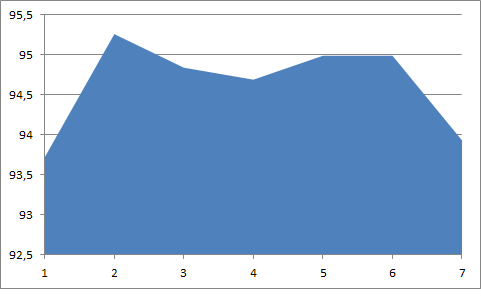
\includegraphics{img/precision-evalContSize_merge.png}
\caption{Precision against evaluation context size, for preprocessing method set to merge of Czech lexical variants and document size set to 3+3}
\end{figure}

 Variance in both sets of results 
is very low, hence there is not much difference in which context size will be used for final evaluation
of all occurrences of polysemous words.


\subsection{ Evaluation on polysemous words of different level}
So far we have been training the model on highly polysemous words, the ones that have 6 or more 
meanings attached to them. Random prediction on these highly polysemous words is very low, therefore
they present a better, more unbiased test set than for instance words that have only 2 meanings, and 
for which random accuracy is 50\%. We will now observe the accuracy of the model set with best
parameters to see how it performs on different sets of words with the same number of meanings. This means
that for instance, in the first column are results of experiments performed on words with 2 meanings attached to them.
Training is performed on the merged set of training and testing development, and testing is done on the unseen set.

\begin{table}[h!]
\begin{tabular}{ l | c c c c c c c  }
     & 2 & 3 & 4 & 5 & 6& 7 & 8  \\
 \hline
Precision  & 92.49 & 97.08 & 87.87 & 97.57 & 64.71 & \textbf{98.49} & 46.15\\ 
Recall & 99.82 & 99.85 & 99.47 & 99.72 & 84.62 & \textbf{99.13} & 60\\ 
Random Precision & 50 & 33.33 & 25 & 20 & 16.67 & 14.29 & 12.5 \\
\end{tabular}
\caption{Precision and Recall of TF--IDF model, closed class filter, document size 1, evaluation context size 3+3 measured against words with different number of meanings}
\end{table} 

\textbf{Conclusion.}\\
We can see that for every group of polysemous words TF--IDF model performs well, where recall is high. The 
lowest scores were noted on words with 6 and 8 meanings, where recall is 84\% and 60\% respectively. Another 
thing that characterizes these low scores is that the test were performed on a low number of instances- there are 
42 instances in the final test set of words with 6 meanings, and only 10 instances of words with 8 meanings. In all other cases number of instances was exceeding 500 test instances, which makes their results a more reliable estimator of the model's accuracy. Precision is reasonably high for all and though it would be expected to be lower 
for words with more meanings, like in the case of words with 7 meanings, out of 508 test instances only 11 were misclassified which resulted with the highest precision on this test set, of  98.49\%.

Overall, it can be said that TF--IFD model performed well at this task. 

\newpage
\section{PMI experiments} 
Experiments with PMI model are like the ones with TF--IDF, grouped in three rounds in order to tune
the model for the best performance. PMI weighting should increase sensitivity of the word to its correct context. 
The theory behind PMI is explained in Chapter 5.4.3.
\begin{itemize}
\item Tuning preprocessing parameters
\item Tuning evaluation context size
\item Evaluation on polysemous words of different level
\end{itemize}
These rounds are ordered sequentially in order to ensure best possible tuning for the model. Final step
represents an evaluation on words with different degree of ambiguity attached to them.


\subsection{Tuning preprocessing parameters}
Being that reasons for using certain values for preprocessing methods parameters were thoroughly described in 
previous section it will not be done again here. From tuning the preprocessing 
parameters for TF--IDF we have a general idea which values for document sizes and preprocessing 
methods give best values. We will thus be concentrating on a smaller set of values for preprocessing parameters. 
Results will be given in summed tables for all preprocessing methods, measured against different 
document sizes.  Other parameters are fixed like in TF--IDF tuning experiments: 
evaluation context size is set to 3, which means that a symmetric window 3 preceding and 3 succeeding words were used to build a vector which was used for classification. The threshold number of meanings was set to 5, which means that every word with the number of sense attached to them that is lower or equal to 5 is discarded from the evaluation. Like before, first was experimented with the individual preprocessing methods. 
Below are given tables for the document size of sentence level. Best results in all the tables are given in bold. 
\begin{table}[h!]
\begin{tabular}{ l | c c | c c | c c | c}
   preprocessing &  1 sentence && 3 sentences && 5 sentences  && random\\
\hline
	& P  &  R & P  &  R & P  &  R &\\
\hline\hline
NO  & 92.31 & 100 & 94.83 & 100 & 95.27 & 100 &  13.96 \\
LOWCASE  & \textbf{98.01} & 100 & 95.01 & 100 & 95.17 & 100 & 13.96  \\
STOP  & 92.31 & 100 & 94.72 & 100 & 93.86 & 100 & 13.96 \\
STEM  & 91.45 & 100 & 91.45 & 100 & 91.45 & 100 & 13.96\\
MERGE  & 92.31 & 100 & 94.83 & 100 & 95.27 & 100 & 13.96 \\
\end{tabular}
\caption{Precision and Recall of PMI model, individual preprocessing methods, sentence level document size}
\end{table}

Total number of not--discarded test set instances was 1174. Random precision was the same for all test cases, as 
was recall (100\%). It seems that lowercasing produced the best result. All other individual preprocessing 
methods achieved slightly better (like the Czech stop word filtering), or slightly worse results (stemming) than with when no preprocessing method was applied to the training set. It is interesting to see that merging of Czech variants brought no improvement whatsoever. Same tests were repeated for the word level document size.

\begin{table}[h!]
\begin{tabular}{ l | c c | c c | c c | c}
   preprocessing &  1+1 word && 2+2 words && 3+3 words && random\\
\hline
	& P  &  R & P  &  R & P  &  R &\\
\hline\hline
NO  & 90.6 & 100 & 94.87 & 100 & 95.73 & 100 & 13.96 \\
LOWCASE  & 94.47 & 100 & \textbf{97.49} & 100 & 97.41 & 100 & 11.47  \\
STOP  & 89.74 & 100 & 93.16 & 100 & 94.87 & 100 & 13.96 \\
STEM  & 90.6 & 100 & 96.58 & 100 & 95.73 & 100 & 13.96\\
 MERGE  & 90.6 & 100 & 94.87 & 100 & 95.73 & 100 & 13.96 \\
\end{tabular}
\caption{Precision and Recall of PMI model, individual preprocessing methods, word level document size}
\end{table}

In the next round of experiments designed for tuning, combinations of preprocessing methods were experimented 
with. First the combinations of methods were tried, for different values of sentence level for document size.

 \begin{table}[h!]
\begin{footnotesize}
\begin{tabular}{ l | c c | c c | c c | c}
   preprocessing &  1 sentence && 3 sentences && 5 sentences  && random\\
\hline
	& P  &  R & P  &  R & P  &  R & precision\\
\hline\hline
 STEM+LOWCASE  & \textbf{98.01} & 100 & 97.93 & 100 & \textbf{98.01} & 100 & 11.47\\
STOP+MERGE  & 92.31 & 100 & 94.72 & 100 & 93.86 & 100 & 13.02 \\
STOP+MERGE+LOWCASE  & 97.84 & 100 & 95.56 & 100 & 94.24 & 100 &11.47\\
STEM+STOP+& 97.93 & 100 & 97.93 & 100 & \textbf{98.01} & 100 & 11.47 \\
+MERGE+LOWCASE  &&&&&&&\\
\end{tabular}
\caption{Precision and Recall using combinations of preprocessing techniques, sentence level document size}
\end{footnotesize}
\end{table}

It seems that the combination of more preprocessing methods achieves an increase in accuracy with the PMI model. Also, It would appear that merging of Czech lexical variants does not contribute in this combination of 
methods. Contrary to it, combinations where lowercasing appears seem to be giving good results. Lowercasing proved its mettle in individual tests of preprocessing methods.  
Then the same test cases were repeated, only this time for the document size word level values. The reason why 
these test cases are repeated is to validate the findings from the previous table. 

 \begin{table}[h!]
\begin{footnotesize}
\begin{tabular}{ l | c c | c c | c c | c}
   preprocessing &  1 sentence && 3 sentences && 5 sentences  && random\\
\hline
	& P  &  R & P  &  R & P  &  R & precision\\
\hline\hline
STEM+LOWCASE  & 95.68 & 100 & \textbf{97.93} & 100 & 97.93 & 100 & 11.47\\
STOP+MERGE  & 89.74 & 100 & 93.16 & 100 & 94.87 & 100 & 13.96 \\
STOP+MERGE+LOWCASE  & 93.95 & 100 & 97.06 & 100 & 97.06 & 100 & 11.47\\
STEM+STOP+ & 95.25 & 100 & 97.93 & 100 & 97.67 & 100 & 11.47 \\
+MERGE+LOWCASE  &&&&&&&\\
\end{tabular}
\caption{Precision and Recall using combinations of preprocessing techniques, word level document size}
\end{footnotesize}
\end{table}


It can be observed that best results for the PMI weighted model are achieved when applying lowercase 
transformation on training and test sets (with the exception of ambiguous words), at the document size set to 
symmetric window of size 3. Test set size was fixed at 1913 instances, out of which 1072 were tested. 
Lowercasing was established to be the best individual preprocessing method (98\% accuracy at the 13\% random 
accuracy, with document size set to 1 sentence). Also in combination with stemming it yielded very good results 
(97.9\& at 12\% random accuracy). With the PMI model, there is general conclusion that combination of 
preprocessing methods actually gives better results. It seems that with reduction of the word space, PMI weights 
become better discriminators of context, when the cosine distance is measured against ambiguous word and its 
context.  

\subsection{Tuning evaluation context size}
Evaluation context size is the size of symmetric window of context which is taken into consideration 
when the polysemous word is encountered during testing. Words that are found within that context
window are used to form a context vector. This context vector's distance is measured against every
vector of each  of the meanings for the polysemous word in question. Sizes of context vector 
experimented with range from 1 to 7. In order to have a larger test set, number of meanings that 
a word can take was lowered to 5 instead of 6 like in the preprocessing experiments. Preprocessing
performed was lowercasing of words, and document size was set to 1 sentence. 
Results are given 
in the table below, and the best result is given in bold. 

\begin{table}[h!]
\begin{tabular}{ l | c c c c c c c}
    &  1+1 & 2+2 & 3+3 & 4+4 & 5+5 & 6+6 & 7+7 \\
\hline
LOWCASE  & 95.54 & 97.75 & \textbf{98.01} & 97.93 & 97.93 & 97.93 & 97.93 \\
\end{tabular}
\caption{Precision and Recall of PMI model,  combined preprocessing methods, word level document size}
\end{table} 

Recall is 100\% for all test cases, therefore it was not displayed in the table. Random prediction is also the same. 
It can be observed that the best evaluation context size is 3+3, and that after it peaks at that point it converges to a stable value for all wider evaluation contexts. 

\textbf{Conclusion.}\\
PMI achieved also very good scores. The best preprocessing method was lowercasing, at 1 sentence document size. The best evaluation context size was found to be 3+3 neighboring words. 


\subsection{ Evaluation on polysemous words of different level}
We will now observe the accuracy of the model set with best
parameters to see how it performs on different sets of words with the same number of meanings. This means
that for instance, in the first column are results of experiments performed on words with 2 meanings attached to them.
Training is performed on the merged set of training and testing development, and testing is done on the unseen set.
\begin{table}[h!]
\begin{tabular}{ l | c c c c c c  }
     & 2 & 3 & 4 & 5 & 6  \\
 \hline
Precision  & 92.17 & 87.39 & 64.85 & 76.77 & 94.55\\ 
Recall & 99.81 & 99.22 & 98.17 & 95 & 96.3\\ 
Random Precision & 50 & 33.33 & 25 & 20 & 16.67 \\
\end{tabular}
\caption{Precision and Recall of PMI model, lowercase preprocessing , document size 1, evaluation context size 3+3 measured against words with different number of meanings}
\end{table} 

PMI model also achieves nice results for all groups of ambiguous terms with different number of meanings. 

\textbf{Conclusion.}\\
It can be seen that PMI model does not provide predictable results when observed while testing on different levels
of ambiguity. For instance, in the Table 6.16 it can be seen that F--measure seems to deteriorate with the number of meanings 
attached for a word starting from 2, but that it jumps again with words that have 6 meanings. 

Overall, it can be said that TF--IFD model performed well at this task. 



\section{RI experiments} 
Random Indexing experiments were performed in order to see how does the matrix reduction influence on the overall accuracy of the algorithm. No weighting was applied on the co--occurrence matrix. The efficacy of the RI to retrieve semantically similar words is very high. 
 The incentive for applying a matrix reduction technique on the WSD task was that the representation of the ambiguous word as a random vector could actually be close in the vector space to a familiar context, that is context in which it often appears. On the other hand, the algorithm should produce low scores for the target word against an unfamiliar context. 
Experiments  with RI model are also, grouped in three rounds in order to tune
the model for the best performance. In the end best model is evaluated on ambiguous words with 
different counts of meanings attached to them.
\begin{itemize}
\item Tuning preprocessing parameters
\item Tuning evaluation context size
\item Evaluation on polysemous words of different level
\end{itemize}

What is different with RI model is that term--document matrix is built incrementally, by adding initially 
assigned pseudo-random vectors of documents to initially pseudo-random vectors of terms. No 
weighting is applied to elements of the matrix. Matrix itself is of much less dimensionality than the 
standard co-occurrence matrix, and is also much less sparse (considerably lower count of zero 
elements). 
 Dimension of random vectors is preset before the construction of matrix and in our 
experiments has that value of 300.

\subsection{Tuning preprocessing parameters}
Like with the models tested before different document sizes and preprocessing methods were tunned
for the best performance of the RI model. 

\begin{table}[h!]
\begin{tabular}{ l | c  | c |c | c}
   preprocessing &  5 sentences & 3 sentences & 1 sentence  & random\\
\hline
	& P  &  P  &  P  &  \\
\hline\hline
 NO  & 69.21  & 70.73  &71.1 & 13.6 \\
LOWCASE  &72.4 & 73.52 & 74.54 &13.6   \\
CLOSED CLASS &70.76 & 72.52 & 76.37 &13.6   \\
STEM+MERGE & 71.5 & 72.21 & 74.19 & 13.6   \\
\end{tabular}
\caption{Precision and Recall of RI model, various preprocessing methods, sentence level document size}
\end{table}

Recall and random prediction were the same for all document sizes, hence they were not displayed in the table above. This aggregated table shows both individual and combined preprocessing methods. Same test cases were 
repeated for the document size of word level. 

\begin{table}[h!]
\begin{tabular}{ l | c  | c |c | c}
   preprocessing &  3+3 words& 2+2 words& 1+1 word& random\\
\hline
	& P  &  P  &  P  &  \\
\hline\hline
NO &  71.36 & 72.51 & 74.37  & 13.6\\
LOWCASE  &72.4 & 73.52 & 74.54 &13.6   \\
CLOSED CLASS & 76.85 &77.33 &78.45 & 13.6\\
STEM+MERGE   & 73.71  & 75.2 & 76.84 &13.6\\
\end{tabular}
\caption{Precision and Recall of RI model, various preprocessing methods, word level document size}
\end{table}


It seems that for RI model smaller document size produces better results. The reason for that can be found in the very nature of term vector generation in RI. Term vectors are constructed from 
superposition of all document vectors it appears in. Document vectors are initially sparse vectors, which
means that the smaller the document size is, the stronger relation gets between a word and its context.
The best model achieved 76.84\% accuracy, with a 100\% Recall, for document size set to 1+1 context
window, and preprocessing method set to filtering of closed--class words.

\subsection{Tuning evaluation context size}
Evaluation context size is the size of symmetric window of context which is taken into consideration 
when the polysemous word is encountered during testing. Words that are found within that context
window are used to form a context vector. This context vector's distance is measured against every
vector of each  of the meanings for the polysemous word in question. Sizes of context vector 
experimented with range from 1 to 7. In order to have a larger test set, number of meanings that 
a word can take was lowered to 5 instead of 6 like in the preprocessing experiments. Preprocessing
performed was lowercasing of words, and document size was set to 1 sentence. 
Results are given 
in the table below, and the best result is given in bold. 

\begin{table}[h!]
\begin{tabular}{ l | c c c c c c c}
    &  1+1 & 2+2 & 3+3 & 4+4 & 5+5 & 6+6 & 7+7 \\
\hline
CLOSED CLASS  & 80.16 & 85.14 & \textbf{86.74} & 79.54 & 79.54& 79.54& 79.54\\
\end{tabular}
\caption{Precision and Recall of RI model,  combined preprocessing methods, word level document size}
\end{table} 

Recall is 100\% for all test cases, therefore it was not displayed in the table. Random prediction is also the same. 
It can be observed that the best evaluation context size is 3+3, and that after it peaks at that point it converges to a stable value for all wider evaluation contexts. 



\subsection{Evaluation on polysemous words of different level}
The best model is evaluated on ambiguous words with 
different counts of meanings attached to them.

\begin{table}[h!]
\begin{tabular}{ l | c c c c c c  }
     & 2 & 3 & 4 & 5 & 6& 7     \\
 \hline
Precision & 87.4 & 86.02 & 84.19 & 76.41 &80.5 & 45.48 \\
Recall   & 95.44 & 98.48 & 94.71 & 95.12 & 100.0 &100.0    \\
Random prediction    & 50 & 33.33 & 25 & 20 & 16.66 & 14.28      \\
\end{tabular}
\caption{Precision and Recall of RI model, closed class filter, document size 1+1, evaluation context size 3+3 measured against words with different number of meanings}
\end{table} 
 It is observable that the best score is achieved with the words that have 3 meanings, but from there precision falls down. It is 
just 45\% for the words with 7 meanings attached to them. Out of all models tested, Random Indexing has the poorest 
performance. One possible explanation is that too much of a contextual information is lost when matrix reduction of the co--
occurrence matrix is performed. As outlined before RI performs well in tasks with the paradigmatic use of context, like in the 
individual word similarity task. However when employed in the WSD task the algorithm is calculating the cosine similarity between the test 
context and all sense candidates for an ambiguous word, where term vectors are extracted from a co-occurrence matrix which has reduced dimensionality. 
It seems that level of contextual information which is vital for the WSD task is lowered as well with the RI matrix reduction, which leads to the poorer performance of the algorithm. 
